\documentclass[a4paper,12pt]{article}
\usepackage{HomeWorkTemplate}

\usepackage[utf8]{inputenc}
\usepackage[]{babel}

\setlength{\parindent}{4em}
\setlength{\parskip}{0.5em}

\renewcommand{\baselinestretch}{1.5}

\usepackage{float} 
\usepackage{caption}
\usepackage{subcaption}
\usepackage{amsmath}
\usepackage[utf8]{inputenc}
\usepackage{lmodern, textcomp}
\usepackage{circuitikz}
\usepackage[shortlabels]{enumitem}
\usepackage{hyperref}
\usepackage{tikz}
\usepackage{amsmath}
\usepackage{amssymb}
\usepackage{tcolorbox}
\usepackage{graphicx}
\usepackage{xepersian}
\settextfont{XB Niloofar}
\usetikzlibrary{arrows,automata}
\usetikzlibrary{circuits.logic.US}
\usepackage{changepage}
\newcounter{problemcounter}
\newcounter{subproblemcounter}
\setcounter{problemcounter}{1}
\setcounter{subproblemcounter}{1}
\newcommand{\problem}[1]
{
	\subsection*{
		پرسش
		\arabic{problemcounter} 
		\stepcounter{problemcounter}
		\setcounter{subproblemcounter}{1}
		#1
	}
}
\newcommand{\subproblem}{
	\textbf{\harfi{subproblemcounter})}\stepcounter{subproblemcounter}
}


\begin{document}
\handout
{اصول پردازش تصویر}
{دکتر مصطفی کمالی تبریزی}
{نیم‌سال اول 1399\lr{-}1400}
{اطلاعیه}
{سیدعلیرضا خادم}
{97100398}
{تمرین سری دوم - سوال سوم}
\section*{موارد لازم.}
برای اجرا لازم است تا تصویر
\lr{books.jpg}
در مسیر
\lr{EX2\_Q3/images/}
قرار داشته باشد.
\section*{روند کلی حل.}
ایده کلی حل سوال پیاده سازی 
\lr{Inverse warping}
و استفاده از آن است.
\section*{توضیح کد.}
برنامه در مجموع حاوی 2 فایل با فرمت
\lr{.py}
می‌باشد که توضیحات هر فایل در پایین آمده است.
\subsection*{$\circ$ utilities.py}
\subsubsection*{\lr{warp\_perspective(src\_image, pts1, width=image\_width)}}
این تابع تصویر 
\lr{src\_image}
و آرایه 
\lr{pst1}
را به عنوان ورودی می‌گیرد. آرایه 
\lr{pst1}
شامل مختطات 4 گوشه کتاب است که به ترتیب گوشه چپ‌بالا، راست‌بالا ، پایین‌چپ و پایین‌راست است.در ابتدا با استفاده از این نقاط طول و عرض کتاب‌ را محاسبه می‌کنیم و بعد توجه به اینکه نسبت ارتفاع به عرض چه مقداری است ارتفاع عکس ریزالت را محاسبه می‌کنیم.(عرض تمامی کتاب‌ها را یکسان و برابر 500 پیکسل در نظر می‌گیرم) بعد با استفاده از تابع آماده‌یِ
\lr{cv.getPerspectiveTransform}
نگاشت
\lr{Perspective}
ای که مجموعه نقاط 
\lr{pts1}
را به 
\lr{pts2}
مپ می‌کند را محاسبه می‌کنیم و با استفاده از 
\lr{np.linalg.inv}
وارون آن را در متغیر
\lr{m\_inverse}
قرار می‌دهد. در ادامه با استفاده از 
\lr{Inverse warping}
و روش درون‌یابی 
\lr{Bilinear}
همانطور که در روابط زیر مشاهده می‌کنید 
\lr{warping}
را انجام می‌دهیم. و در نهایت نتیجه را به عنوان خروجی برمی‌گرداند.
\begin{figure}[H]
	\centering
	\begin{subfigure}{0.9\textwidth}
		\centering
		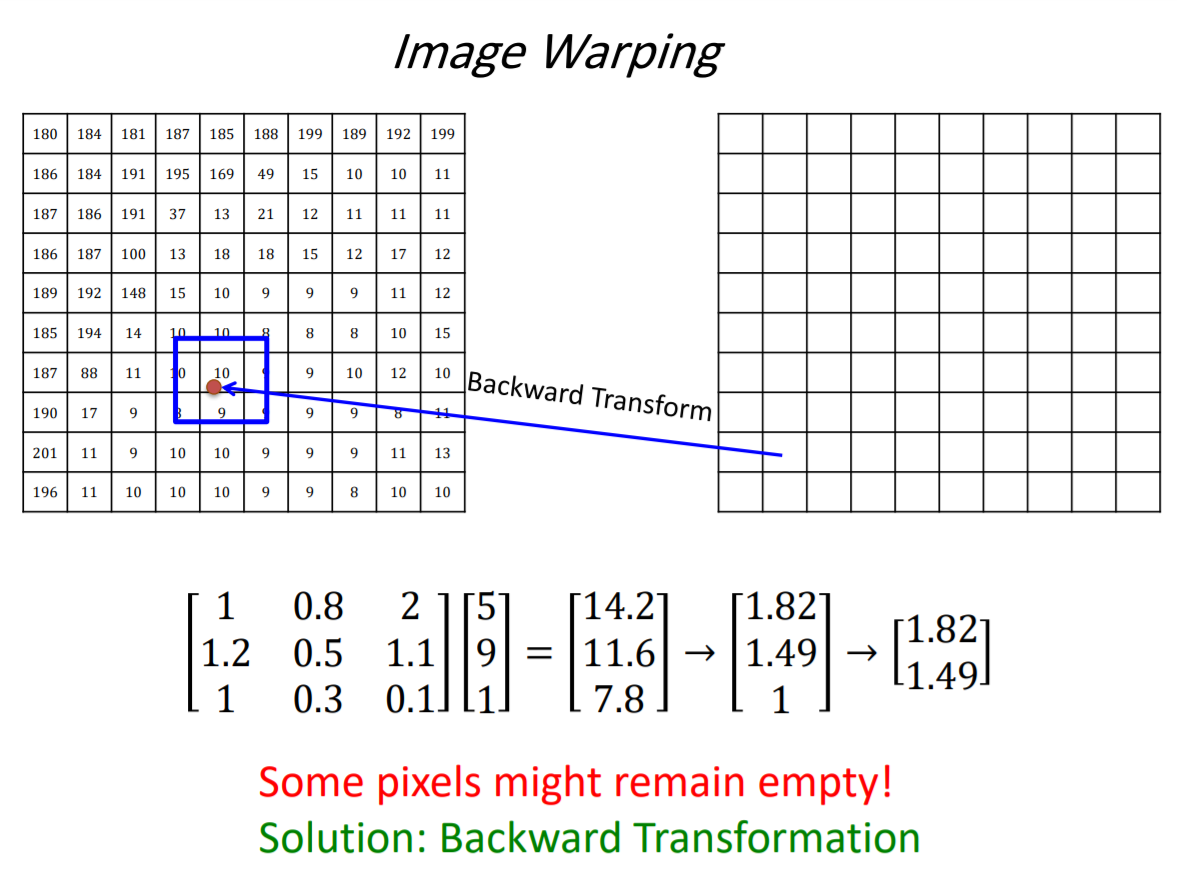
\includegraphics[width=\textwidth]{1.png}
	\end{subfigure}
	\begin{subfigure}{0.9\textwidth}
		\centering
		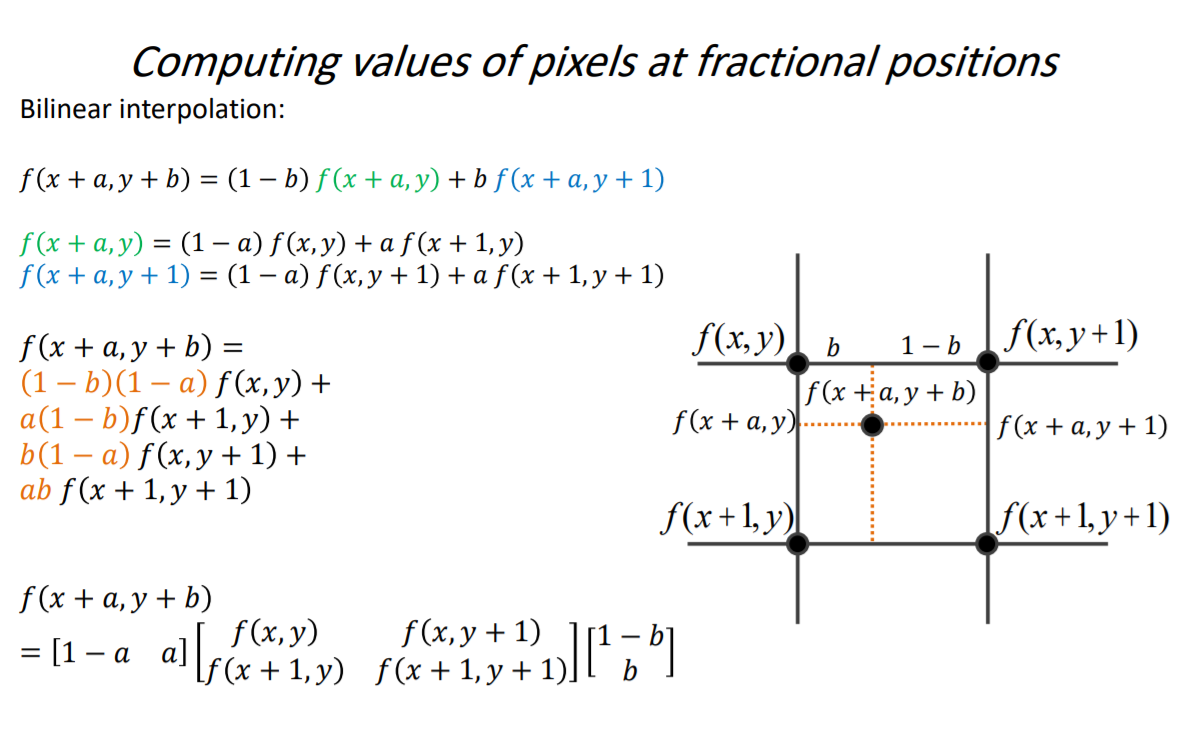
\includegraphics[width=\textwidth]{2.png}
	\end{subfigure}
\end{figure}

\subsection*{$\circ$ q3.py}
در این فایل ابتدا تصویر کتاب‌ها لود شده است و سپس دیتای مربوط به مختصات گوشه‌های کتاب‌ها است و در سه فایل مجزا قرار گرفته است لود می‌شود و در ادامه با استفاده از این داده‌ها و با استفاده از 
\lr{warp\_perspective}
عمل
\lr{warping}
انجام شده و نتایج در 
\lr{res04.jpg}
،
\lr{res04.jpg}
و
\lr{res05.jpg}
و در مسیر
\lr{EX2\_Q3/results/}
ذخیره شده است.

\end{document}
